% !TEX root=ricardo_draft.tex

\begin{figure}[!th]
\begin{center}
\vspace{-1ex}
\centerline{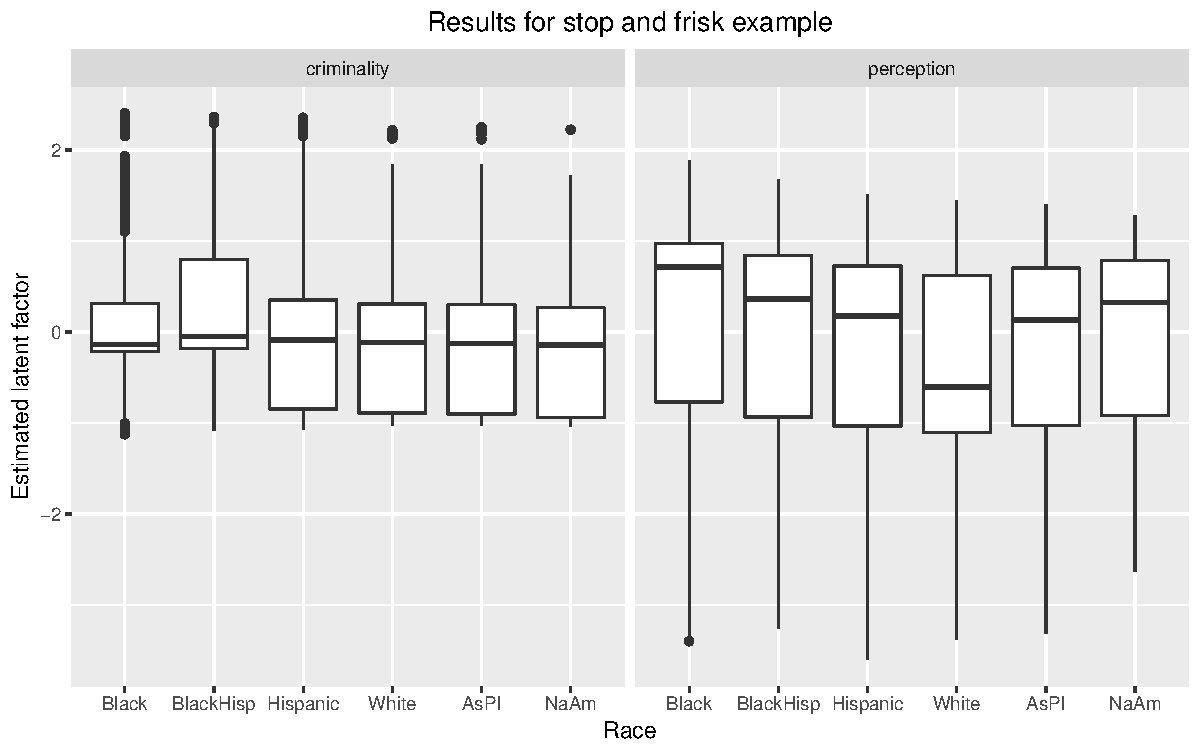
\includegraphics[width=\columnwidth]{stopandfrisk_output.pdf}}
\vspace{-2ex}
\caption{Distributions of estimated latent perception and criminality scores for the stop and frisk dataset.\label{figure.stop_and_frisk_output}\vspace{-5ex}}
\vspace{-2ex}
\end{center}
\end{figure}

In this section we evaluate our framework for modeling fairness. We test our approach on two practical problems in which fairness must be enforced. For each problem we construct causal models, and make explicit how unfairness may affect observed and unobserved variables in the world. Given these models we are able to (a) derive counterfactually fair predictors and (b) predict latent variables such as a person's `criminality' (which may be useful for predicting crime) as well as their `perceived criminality' (which may be due to prejudices based on race and gender). We analyze how realistic our models are by comparing our observations with data generated from the model. We consider two real-world problems, the first is \emph{fair prediction of success in law school} and the second is \emph{separating actual and perceived criminality in stop-and-frisk data}.

\subsection{Law school success}
\label{sec:law-school-success}
From 1991 to 1996 the Law School Admission Council
counducted a longitudinal survey following students across 163 law
schools in the United States \cite{wightman1998lsac}. % The survey was
% designed to assess `the law school experience of minority students, as
% well as their ultimate entry into the profession'.
The survey contains students' features before entering law school
including: their entrance exam scores (LSAT) and their grade-point
average (GPA) and the average grade of their first year of law school
(FYA). %, and following Law
%School i.e. whether students passed the final examination, the `bar
%exam' (P)).

Given this data a law school may wish to predict if a law student
will succeed in their first year (have a high FYA) from information about their academic performance 
before law school. The school would also like to make sure
these predictions are not biased by an individual's race and
sex. However, the observed information about
students, the LSAT, GPA, and FYA scores,  may be biased due to 
social factors relating to race and gender. We explicitly model these
``unfair'' factors alongside a latent variable that is counterfactually
fair.

\paragraph{Counterfactually fair prediction.}
As described in Section 5.1 there are three ways in which we can model a counterfactually fair predictor of FYA: 1. We can use any features which are not descendants of race and gender for prediction; 2. We can model latent `fair' variables which are parents of observed variables. Crucially, these variables are independent of race and gender; 3. We can model the data using an additive error model, and use the independent error terms for making predictions of FYA. These models use increasingly strong assumptions that corresponds to a trade-off for lower predictive error.

First we note that because we suspect LSAT, GPA, and FYA to all be biased by race and sex, we cannot use any observed features to construct a counterfactually fair predictor as described in method one. Instead we would need to resort to a constant predictor, such as the mean of FYA over the training set. As this model is trivial we do not consider it. 

Following the second approach, we postulate that a latent variable: a student's \emph{knowledge} (K), affects GPA, LSAT, and FYA scores. The causal graph corresponding to this model is shown in Figure~\ref{figure.law_school}. This model is a short-hand for a system of equations:

\begin{align}
\mbox{GPA} &\sim {\cal N}(b_{G} + w_{G}^K K + w_{G}^R R + w_{G}^S S, \sigma_{G}) \nonumber \\
\mbox{LSAT} &\sim \textrm{Poisson}(\exp(b_{L} + w_{L}^K K + w_{L}^R R + w_{L}^S S)) \nonumber \\
\mbox{FYA} &\sim {\cal N}(w_{F}^K K + w_{F}^R R + w_{F}^S S, 1) \nonumber \\
K &\sim {\cal N}(0,1) \nonumber
\end{align}
We can perform inference on this model using an observed training set to get an estimate of the posterior distribution of $K$. We call the predictor constructed using $K$ \emph{Fair, Level 2}.

In the third approach, we model GPA, LSAT, and FYA as continuous variables with additive error terms independent of race and sex (they may in turn be correlated with each other). This model is shown in Figure


% impacts these features.

% We propose to model the law school data as shown in
% Figure~\ref{figure.law_school}. We suspect that variables race and sex
% affect student performance (e.g. GPA, LSAT, and FYA) due to factors
% such as cultural norms, which assume that individuals of a certain
% race or gender are `better suited' to be lawyers. Such beliefs could
% adversely impact students who do not fit these norms. Instead we would
% like to model the latent \emph{knowledge} (K) of a student, which also
% impacts these features. 
% We can then construct a predictor that
% predicts FYA fairly using knowledge. It is easy to show that such a predictor
% is counterfactually fair, whereas a predictor that uses features GPA and
% LSAT is not (in this case even including race and sex as
% features cannot correct this, as can be done in the linear case). The
% causal 
 %; %3. \textbf{Variational Fair Autoencoder (VFAE)} \cite{louizos2015variational}, a recent approach that works to learn a fair representation of the original data.
% compute counterfactuals for both race and gender



\paragraph{Accuracy.}
We compare the RMSE of all methods for predicting FYA on a hold out dataset in Table~\ref{table.pred_law}. For our method we only use samples from the posterior of knowledge for prediction. As we believe FYA is affected by race and sex note that any model that wishes to be fair w.r.t. to these variables must necessarily lose prediction accuracy. We see this Table~\ref{table.pred_law}: the full model achieves the lowest RMSE as it is able to reconstruct additional information about FYA using race and sex. We note that our method is able to achieve nearly the same RMSE as the unaware model. This implies that our knowledge variable is nearly as good as the unfair variables GPA and LSAT at reconstructing FYA.


\paragraph{Counterfactual fairness.}
We would like to empirically test whether the baseline methods are counterfactually fair. Because we do not know the true model of the data, we propose to use Figure~\ref{figure.law_school} as our model of the real world. If this describes the true world we can evaluate counterfactual fairness easily: we can simply sample from the model while fixing an individual's race/sex to particular values. By changing race/sex we can obtain the counterfactual values $\mbox{GPA}_a,\mbox{GPA}_{a'}$ where $a,a'$ are different values of race/sex (and similarly for LSAT). We compare how predictions of FYA change when using counterfactual features versus the original sampled features. Figure~\ref{figure.counterfactual} shows how the distribution of predicted FYA changes when race, sex, and both race and sex are changed (for race, as the majority of individuals have marked their race as white or black we just consider counterfactuals for this subset of individuals).

% here describe what we see

% maybe sample from model and check it out
%\paragraph{Model validity.}
 

% TODO rank top 10 students by ability or by other score in law_school.py which only considers observed features

\begin{figure}[th]
\begin{center}
\vspace{-1ex}
\centerline{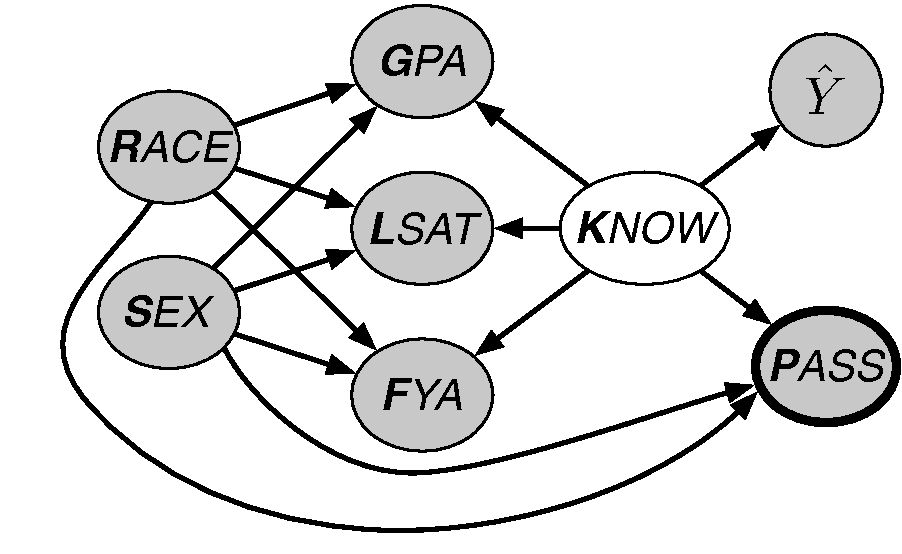
\includegraphics[width=0.8\columnwidth]{law_school_model}}
\vspace{-2ex}
\caption{A causal model for the problem of predicting law school success fairly.\label{figure.law_school}\vspace{-2ex}}
\vspace{-2ex}
\end{center}
\end{figure}


\begin{figure}[th]
\begin{center}
 \label{figure.counterfactual}
\vspace{-1ex}
\centerline{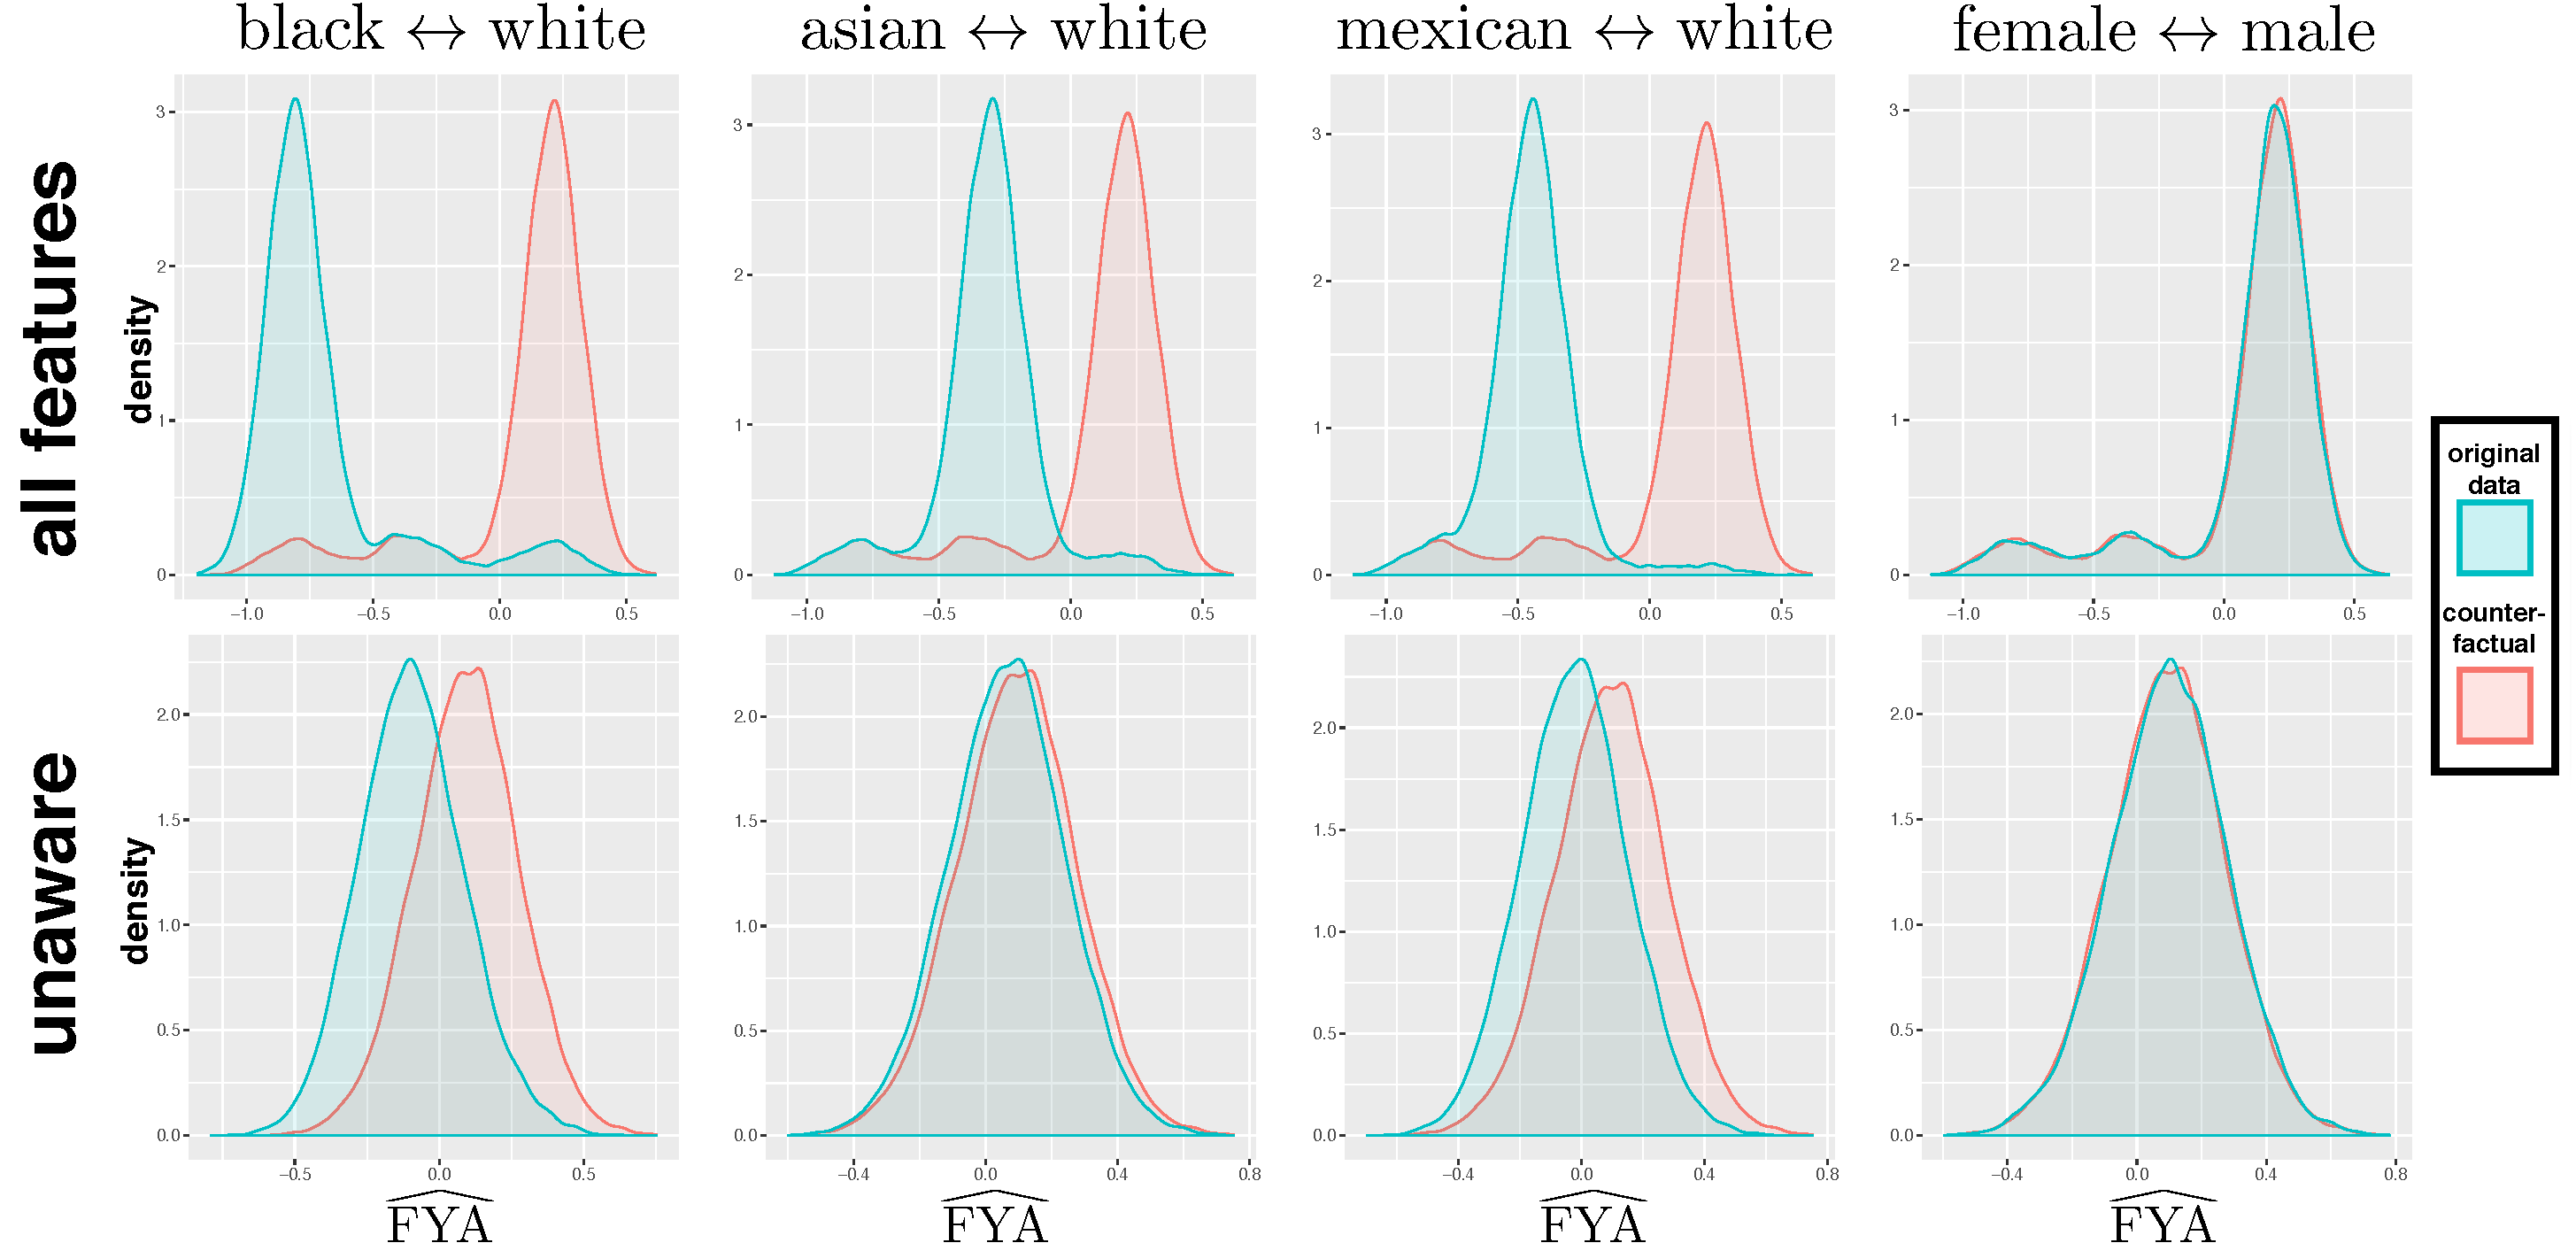
\includegraphics[width=\columnwidth]{counterfactual}}
\vspace{-2ex}
\caption{Density plots of predicted $\mbox{FYA}_a$ and $\mbox{FYA}_{a'}$.}
\vspace{-2ex}
\end{center}
\end{figure}


% \begin{table}[t]
% \vspace{-2ex}
% \caption{}
% \vspace{-3ex}
% \label{table.pred_law}
% \begin{center}
% \resizebox{\columnwidth}{!}
% {
% \begin{sc}
% \footnotesize
% \begin{tabular}{c|c|c|c}
% \hline
% %\multicolumn{5}{c}{\textbf{Lower Bounds}}\\
% \hline
% & full & unaware  & fair l2 & fair l3 \\
% \hline
% RMSE & 0.873 & 0.894 & 0.929 & 0.918 \\ \hline
% \end{tabular}
% \end{sc}
% }
% \end{center}
% \vspace{-4ex}
% \end{table}

%{lr@{$\pm$}lr@{$\pm$}lr@{$\pm$}l}
\begin{table}
\centering
\caption{Prediction results using logistic regression. Note that we must sacrifice a small amount of accuracy to ensuring counterfactually fair prediction (fair), versus the model which uses all features, including race and sex (unfair).}\label{table.pred_law}
\begin{tabular}{ccccc} 
\hline
 &  {\bf Full} & {\bf Unaware} & {\bf Fair L2} & {\bf Fair L3} \\
\hline
RMSE & 0.873 & 0.894 & 0.929 & 0.918 \\
%\bf{Method} & %\multicolumn{2}{c}{\bf Full} & \multicolumn{2}{c}{\bf Unaware} & \multicolumn{2}{c}{\bf Fair L2} & \multicolumn{2}{c}{\bf Fair L3} \\
\hline
\end{tabular}
\end{table}



\subsection{True vs. Perceived Criminality}
\label{sec:true-vs.-perceived}
Every year since 2002, the New York Police Department (NYPD) has recorded information about every time a police officer has stopped someone. The officer records information such as if they searched or frisked the individual, whether a weapon was found, the individual's appearance, whether force was used, etc. We look at this data collected during 2014 for our analysis.

\paragraph{Model.}
We model this stop-and-frisk data using the graph in Figure~\ref{figure.stop_and_frisk}. Specifically, we posit main causes for the observations: \emph{Arrest} (if an individual was arrested), \emph{Summons} (an individual was called to a court-summons), \emph{Weapon} (an individual was found to be carrying a weapon), \emph{Force} (some sort of force was used during the stop), \emph{Frisked}, and \emph{Searched}. The first cause of these observations is some measure of an individual's latent \emph{Criminality}, which we do not observe. We believe there is an additional cause, an individual's perceived criminality, \emph{Perception}, also unobserved. This second factor is introduced as we have reason


\begin{figure}[th]
\begin{center}
\vspace{-1ex}
\centerline{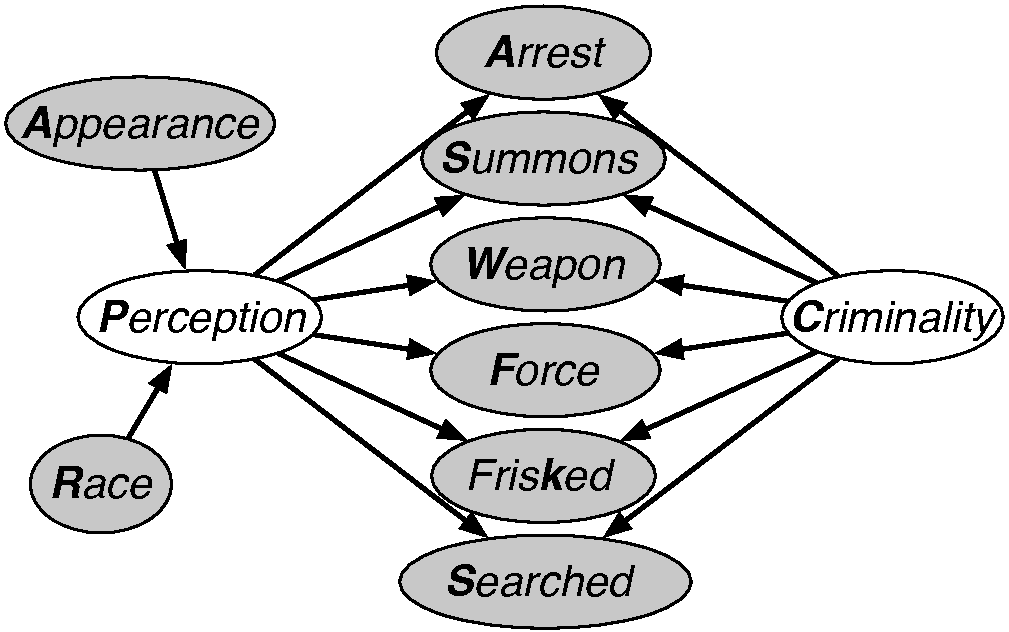
\includegraphics[width=\columnwidth]{stop_and_frisk_model3.pdf}}
\vspace{-2ex}
\caption{A causal model for the stop and frisk dataset.\label{figure.stop_and_frisk}\vspace{-4ex}}
\vspace{-2ex}
\end{center}
\end{figure}


%\subsection{Model criticism}
%%% Local Variables:
%%% mode: latex
%%% TeX-master: "ricardo_draft"
%%% End:
